\documentclass[11pt,ignorenonframetext,]{beamer}
\setbeamertemplate{caption}[numbered]
\setbeamertemplate{caption label separator}{: }
\setbeamercolor{caption name}{fg=normal text.fg}
\beamertemplatenavigationsymbolsempty
\usepackage{lmodern}
\usepackage{amssymb,amsmath}
\usepackage{ifxetex,ifluatex}
\usepackage{fixltx2e} % provides \textsubscript
\ifnum 0\ifxetex 1\fi\ifluatex 1\fi=0 % if pdftex
  \usepackage[T1]{fontenc}
  \usepackage[utf8]{inputenc}
\else % if luatex or xelatex
  \ifxetex
    \usepackage{mathspec}
  \else
    \usepackage{fontspec}
  \fi
  \defaultfontfeatures{Ligatures=TeX,Scale=MatchLowercase}
\fi
\usetheme[]{metropolis}
% use upquote if available, for straight quotes in verbatim environments
\IfFileExists{upquote.sty}{\usepackage{upquote}}{}
% use microtype if available
\IfFileExists{microtype.sty}{%
\usepackage{microtype}
\UseMicrotypeSet[protrusion]{basicmath} % disable protrusion for tt fonts
}{}
\newif\ifbibliography
\hypersetup{
            pdftitle={Lecture 23},
            pdfauthor={Colin Rundel},
            pdfborder={0 0 0},
            breaklinks=true}
\urlstyle{same}  % don't use monospace font for urls
\usepackage{color}
\usepackage{fancyvrb}
\newcommand{\VerbBar}{|}
\newcommand{\VERB}{\Verb[commandchars=\\\{\}]}
\DefineVerbatimEnvironment{Highlighting}{Verbatim}{commandchars=\\\{\}}
% Add ',fontsize=\small' for more characters per line
\newenvironment{Shaded}{}{}
\newcommand{\KeywordTok}[1]{\textcolor[rgb]{0.00,0.44,0.13}{\textbf{#1}}}
\newcommand{\DataTypeTok}[1]{\textcolor[rgb]{0.56,0.13,0.00}{#1}}
\newcommand{\DecValTok}[1]{\textcolor[rgb]{0.25,0.63,0.44}{#1}}
\newcommand{\BaseNTok}[1]{\textcolor[rgb]{0.25,0.63,0.44}{#1}}
\newcommand{\FloatTok}[1]{\textcolor[rgb]{0.25,0.63,0.44}{#1}}
\newcommand{\ConstantTok}[1]{\textcolor[rgb]{0.53,0.00,0.00}{#1}}
\newcommand{\CharTok}[1]{\textcolor[rgb]{0.25,0.44,0.63}{#1}}
\newcommand{\SpecialCharTok}[1]{\textcolor[rgb]{0.25,0.44,0.63}{#1}}
\newcommand{\StringTok}[1]{\textcolor[rgb]{0.25,0.44,0.63}{#1}}
\newcommand{\VerbatimStringTok}[1]{\textcolor[rgb]{0.25,0.44,0.63}{#1}}
\newcommand{\SpecialStringTok}[1]{\textcolor[rgb]{0.73,0.40,0.53}{#1}}
\newcommand{\ImportTok}[1]{#1}
\newcommand{\CommentTok}[1]{\textcolor[rgb]{0.38,0.63,0.69}{\textit{#1}}}
\newcommand{\DocumentationTok}[1]{\textcolor[rgb]{0.73,0.13,0.13}{\textit{#1}}}
\newcommand{\AnnotationTok}[1]{\textcolor[rgb]{0.38,0.63,0.69}{\textbf{\textit{#1}}}}
\newcommand{\CommentVarTok}[1]{\textcolor[rgb]{0.38,0.63,0.69}{\textbf{\textit{#1}}}}
\newcommand{\OtherTok}[1]{\textcolor[rgb]{0.00,0.44,0.13}{#1}}
\newcommand{\FunctionTok}[1]{\textcolor[rgb]{0.02,0.16,0.49}{#1}}
\newcommand{\VariableTok}[1]{\textcolor[rgb]{0.10,0.09,0.49}{#1}}
\newcommand{\ControlFlowTok}[1]{\textcolor[rgb]{0.00,0.44,0.13}{\textbf{#1}}}
\newcommand{\OperatorTok}[1]{\textcolor[rgb]{0.40,0.40,0.40}{#1}}
\newcommand{\BuiltInTok}[1]{#1}
\newcommand{\ExtensionTok}[1]{#1}
\newcommand{\PreprocessorTok}[1]{\textcolor[rgb]{0.74,0.48,0.00}{#1}}
\newcommand{\AttributeTok}[1]{\textcolor[rgb]{0.49,0.56,0.16}{#1}}
\newcommand{\RegionMarkerTok}[1]{#1}
\newcommand{\InformationTok}[1]{\textcolor[rgb]{0.38,0.63,0.69}{\textbf{\textit{#1}}}}
\newcommand{\WarningTok}[1]{\textcolor[rgb]{0.38,0.63,0.69}{\textbf{\textit{#1}}}}
\newcommand{\AlertTok}[1]{\textcolor[rgb]{1.00,0.00,0.00}{\textbf{#1}}}
\newcommand{\ErrorTok}[1]{\textcolor[rgb]{1.00,0.00,0.00}{\textbf{#1}}}
\newcommand{\NormalTok}[1]{#1}
\usepackage{graphicx,grffile}
\makeatletter
\def\maxwidth{\ifdim\Gin@nat@width>\linewidth\linewidth\else\Gin@nat@width\fi}
\def\maxheight{\ifdim\Gin@nat@height>\textheight0.8\textheight\else\Gin@nat@height\fi}
\makeatother
% Scale images if necessary, so that they will not overflow the page
% margins by default, and it is still possible to overwrite the defaults
% using explicit options in \includegraphics[width, height, ...]{}
\setkeys{Gin}{width=\maxwidth,height=\maxheight,keepaspectratio}

% Prevent slide breaks in the middle of a paragraph:
\widowpenalties 1 10000
\raggedbottom

\AtBeginPart{
  \let\insertpartnumber\relax
  \let\partname\relax
  \frame{\partpage}
}
\AtBeginSection{
  \ifbibliography
  \else
    \let\insertsectionnumber\relax
    \let\sectionname\relax
    \frame{\sectionpage}
  \fi
}
\AtBeginSubsection{
  \let\insertsubsectionnumber\relax
  \let\subsectionname\relax
  \frame{\subsectionpage}
}

\setlength{\parindent}{0pt}
\setlength{\parskip}{6pt plus 2pt minus 1pt}
\setlength{\emergencystretch}{3em}  % prevent overfull lines
\providecommand{\tightlist}{%
  \setlength{\itemsep}{0pt}\setlength{\parskip}{0pt}}
\setcounter{secnumdepth}{0}

\usepackage{geometry}
\usepackage{graphicx}
\usepackage{amssymb}
\usepackage{color}          	% gives color options
\usepackage{url}		% produces hyperlinks
\usepackage[english]{babel}
\usepackage{colortbl}	% allows for color usage in tables
\usepackage{multirow}	% allows for rows that span multiple rows in tables
\usepackage{xcolor}		% this package has a variety of color options
\usepackage{calc}
\usepackage{multicol}
\usepackage{wrapfig}
\usepackage{textcomp}
\usepackage{bm}
\usepackage{bbm}
\usepackage{setspace}
\usepackage{changepage}
\usepackage{isotope}
\singlespacing

\usepackage{fontspec}
\newfontfamily\DejaSans{DejaVu Sans}

%%%%%%%%%%%%%%%%
% Small code output
%%%%%%%%%%%%%%%%

%% change fontsize of R code

\makeatletter
\@ifundefined{Shaded}{\newenvironment{Shaded}{}{}}{}
\makeatother


\let\oldShaded\Shaded
\let\endoldShaded\endShaded
\renewenvironment{Shaded}{\footnotesize\begin{spacing}{0.9}\oldShaded}{\endoldShaded\end{spacing}}

%% change fontsize of output
\let\oldverbatim\verbatim
\let\endoldverbatim\endverbatim
\renewenvironment{verbatim}{\footnotesize\begin{spacing}{0.9}\oldverbatim}{\endoldverbatim\end{spacing}}


\newcommand{\tinyoutput}{
  \renewenvironment{Shaded}{\tiny\begin{spacing}{0.9}\oldShaded}{\endoldShaded\end{spacing}}
  \renewenvironment{verbatim}{\tiny\begin{spacing}{0.9}\oldverbatim}{\endoldverbatim\end{spacing}}
}

\newcommand{\scriptoutput}{
  \renewenvironment{Shaded}{\scriptsize\begin{spacing}{0.9}\oldShaded}{\endoldShaded\end{spacing}}
  \renewenvironment{verbatim}{\scriptsize\begin{spacing}{0.9}\oldverbatim}{\endoldverbatim\end{spacing}}
}

\newcommand{\footnoteoutput}{
  \renewenvironment{Shaded}{\footnotesize\begin{spacing}{0.9}\oldShaded}{\endoldShaded\end{spacing}}
  \renewenvironment{verbatim}{\footnotesize\begin{spacing}{0.9}\oldverbatim}{\endoldverbatim\end{spacing}}
}

%\newcommand{\verbatimfont}[1]{\renewcommand{\verbatim@font}{\ttfamily#1}}


%%%%%%%%%%%%%%%%
% Custom Colors
%%%%%%%%%%%%%%%%

\definecolor{redhl}{rgb}{0.98,0.29,0.28}
\definecolor{yellowhl}{rgb}{0.98,0.87,0.28}
\newcommand{\hlr}[1]{\fcolorbox{redhl}{white}{$\displaystyle #1$}}
\newcommand{\hly}[1]{\fcolorbox{yellowhl}{white}{$\displaystyle #1$}}

\newcommand{\vvfill}{\vskip0pt plus 1filll}


\xdefinecolor{oiBlue}{rgb}{0.15, 0.35, 0.55}
\xdefinecolor{gray}{rgb}{0.5, 0.5, 0.5}
\xdefinecolor{darkGray}{rgb}{0.3, 0.3, 0.3}
\xdefinecolor{darkerGray}{rgb}{0.2, 0.2, 0.2}
\xdefinecolor{rubineRed}{rgb}{0.89,0,0.30}
\xdefinecolor{linkCol}{rgb}{0.11,0.49,0.95}	
\xdefinecolor{irishGreen}{rgb}{0,0.60,0}	
\xdefinecolor{darkturquoise}{rgb}{0.44, 0.58, 0.86}
\definecolor{lightGreen}{rgb}{0.533,0.765,0.42}
%\xdefinecolor{hlblue}{rgb}{0.051,0.65,1}
\xdefinecolor{hlblue}{rgb}{ 0.055, 0.639, 0.831}
\definecolor{light}{rgb}{.337,.608,.741}
\definecolor{dark}{rgb}{.337,.608,.741}

\definecolor{cpink}{rgb}{0.93, 0.23, 0.51}

%%%%%%%%%%%%%%%%
% Custom Commands
%%%%%%%%%%%%%%%%

% text colors
\newcommand{\red}[1]{\textit{\textcolor{rubineRed}{#1}}}
\newcommand{\orange}[1]{\textit{\textcolor{orange}{#1}}}
\newcommand{\pink}[1]{\textit{\textcolor{rubineRed!90!white!50}{#1}}}
\newcommand{\green}[1]{\textit{\textcolor{irishGreen}{#1}}}
\newcommand{\blue}[1]{\textit{\textcolor{darkturquoise}{#1}}}
\newcommand{\light}[1]{\textcolor{light}{\textbf{#1}}}
\newcommand{\dark}[1]{\textcolor{dark}{#1}}
\newcommand{\gray}[1]{\textcolor{gray}{#1}}


% links: webURL, webLin, appLink
\newcommand{\webURL}[1]{\urlstyle{same}{\textit{\textcolor{linkCol}{\url{#1}}} }}
\newcommand{\webLink}[2]{\href{#1}{\textcolor{linkCol}{{#2}}}}
\newcommand{\appLink}[2]{\href{#1}{\textcolor{lightGreen!80!black!90}{{#2}}}}

% mail
\newcommand{\mail}[1]{\href{mailto:#1}{\textit{\textcolor{linkCol}{#1}}}}

% highlighting: hl, hlGr, mathhl
\newcommand{\hl}[1]{\textit{\textcolor{hlblue}{#1}}}
\newcommand{\hlGr}[1]{\textit{\textcolor{lightGreen}{#1}}}
\newcommand{\hlRd}[1]{\textit{\textcolor{rubineRed}{#1}}}
\newcommand{\mathhl}[1]{\textcolor{hlblue}{\ensuremath{#1}}}

% example
\newcommand{\ex}[1]{\textcolor{blue}{{{\small (#1)}}}}


\DeclareMathOperator*{\argmin}{arg\,min}
\DeclareMathOperator*{\argmax}{arg\,max}

\title{Lecture 23}
\subtitle{Spatio-temporal Models}
\author{Colin Rundel}
\date{04/17/2017}

\begin{document}
\frame{\titlepage}

\section{Spatial Models with AR time
dependence}\label{spatial-models-with-ar-time-dependence}

\begin{frame}[fragile]{Example - Weather station data}

\footnotesize

Based on Andrew Finley and Sudipto Banerjee's notes from
\href{http://blue.for.msu.edu/NEON/SC/}{National Ecological Observatory
Network (NEON) Applied Bayesian Regression Workshop, March 7 - 8, 2013}
\href{http://blue.for.msu.edu/NEON/SC/exercises/exercise-6/initial-exploration-spDynLM.pdf}{Module
6}

\texttt{NETemp.dat} - Monthly temperature data (Celsius) recorded across
the Northeastern US starting in January 2000.

\scriptoutput

\begin{Shaded}
\begin{Highlighting}[]
\KeywordTok{library}\NormalTok{(spBayes)}
\KeywordTok{data}\NormalTok{(}\StringTok{"NETemp.dat"}\NormalTok{)}
\NormalTok{ne_temp =}\StringTok{ }\NormalTok{NETemp.dat }\OperatorTok
\StringTok{  }\KeywordTok{filter}\NormalTok{(UTMX }\OperatorTok{>}\StringTok{ }\FloatTok{5.5e6}\NormalTok{, UTMY }\OperatorTok{>}\StringTok{ }\FloatTok{3e6}\NormalTok{) }\OperatorTok
\StringTok{  }\KeywordTok{select}\NormalTok{(}\DecValTok{1}\OperatorTok{:}\DecValTok{27}\NormalTok{) }\OperatorTok
\StringTok{  }\KeywordTok{tbl_df}\NormalTok{()}
\NormalTok{ne_temp}
\NormalTok{## # A tibble: 34 × 27}
\NormalTok{##     elev    UTMX    UTMY        y.1       y.2        y.3      y.4       y.5}
\NormalTok{##    <int>   <dbl>   <dbl>      <dbl>     <dbl>      <dbl>    <dbl>     <dbl>}
\NormalTok{## 1    102 6094162 3195181  -6.388889 -3.611111  3.7222222 6.777778 12.555556}
\NormalTok{## 2      1 6245390 3262354  -6.277778 -4.111111  2.6111111 6.555556 11.388889}
\NormalTok{## 3    157 6157302 3484043 -11.111111 -9.444444 -0.3888889 3.944444  9.888889}
\NormalTok{## 4    176 6123610 3527665 -11.611111 -9.722222 -1.1666667 2.888889  9.666667}
\NormalTok{## 5    400 6004871 3275456 -12.611111 -9.055556 -1.6111111 2.555556  8.555556}
\NormalTok{## 6    133 6051946 3225830  -9.111111 -6.388889  1.2222222 4.944444 10.888889}
\NormalTok{## 7     56 6099462 3184587  -7.944444 -6.055556  2.0555556 5.555556 11.111111}
\NormalTok{## 8     59 6074601 3136288  -6.555556 -3.500000  3.1666667 6.166667 11.500000}
\NormalTok{## 9    160 6174891 3455064  -9.944444 -8.944444 -0.2777778 3.555556  9.611111}
\NormalTok{## 10   360 6005282 3327413 -12.277778 -9.444444 -1.5000000 2.944444  9.000000}
\NormalTok{## # ... with 24 more rows, and 19 more variables: y.6 <dbl>, y.7 <dbl>,}
\NormalTok{## #   y.8 <dbl>, y.9 <dbl>, y.10 <dbl>, y.11 <dbl>, y.12 <dbl>, y.13 <dbl>,}
\NormalTok{## #   y.14 <dbl>, y.15 <dbl>, y.16 <dbl>, y.17 <dbl>, y.18 <dbl>, y.19 <dbl>,}
\NormalTok{## #   y.20 <dbl>, y.21 <dbl>, y.22 <dbl>, y.23 <dbl>, y.24 <dbl>}
\end{Highlighting}
\end{Shaded}

\end{frame}

\begin{frame}{}

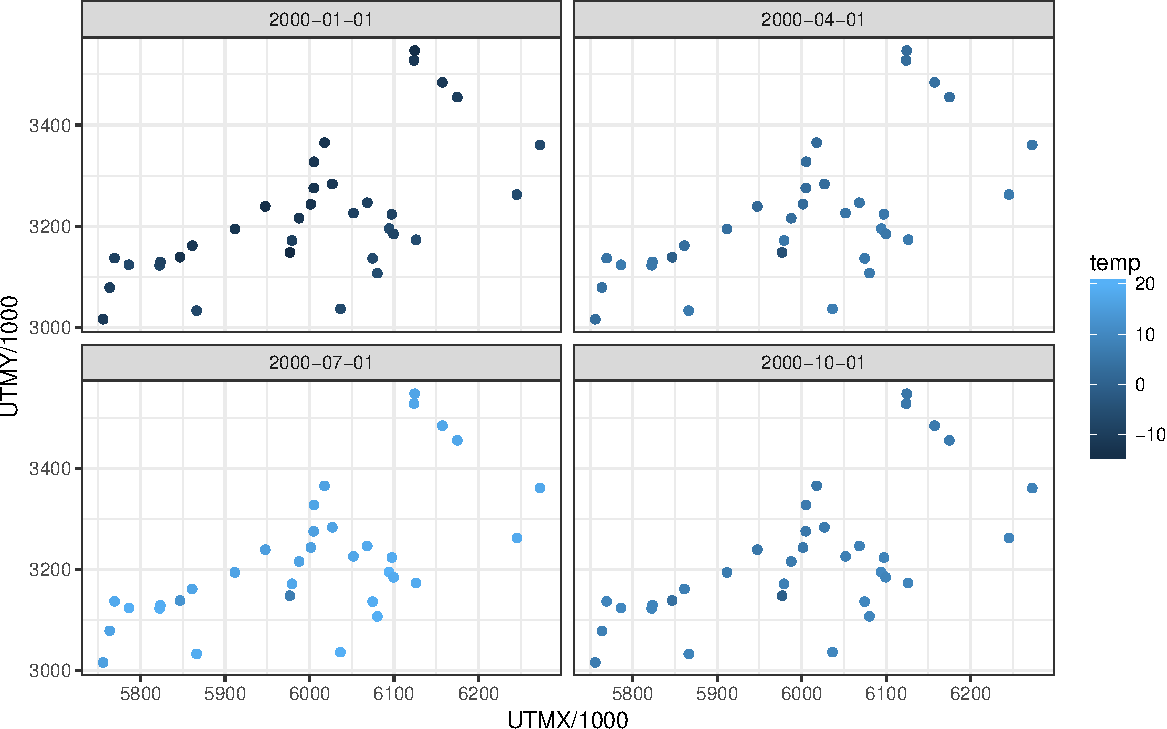
\includegraphics{Lec23_files/figure-beamer/unnamed-chunk-2-1.pdf}

\end{frame}

\begin{frame}{Dynamic Linear / State Space Models (time)}

\[ 
\begin{aligned}
{{y}_t} &= \underset{1 \times p}{\bm{F}'_t} ~ \underset{p \times 1}{\bm{\theta}_t} + {{v}_t} 
&\qquad\qquad\text{observation equation}\\
\underset{p\times 1}{\bm\theta_t} &= \underset{p \times p}{\bm{G}_t} ~ \underset{p \times 1}{\bm\theta}_{t-1} + \underset{p \times 1}{\bm\omega_t}
&\qquad\qquad\text{evolution equation}\\
\end{aligned}
\]

\[ 
\begin{aligned}
\bm{v}_t &\sim \mathcal{N}(0,\bm{V}_t) \\
\bm\omega_t &\sim \mathcal{N}(0,\bm{W}_t) \\
\end{aligned}
\]

\end{frame}

\begin{frame}[t]{DLM vs ARMA}

ARMA / ARIMA are a special case of a dynamic linear model, for example
an \(AR(p)\) can be written as \[ F_t' = (1, 0, \ldots, 0) \]
\[ G_t = \begin{pmatrix}
\phi_1 & \phi_2 & \cdots & \phi_{p-1} & \phi_p \\
1      & 0      & \cdots & 0          & 0      \\
0      & 1      & \cdots & 0          & 0      \\
\vdots & \vdots & \ddots & \vdots     & 0      \\
0      & 0      & \cdots & 1          & 0      \\
\end{pmatrix}\] \[ \begin{aligned}
\omega_t &= (\omega_1, 0, \ldots 0), 
\quad &\omega_1 \sim \mathcal{N}(0,\,\sigma^2)
\end{aligned}
\]

\pause

\vspace{2mm}

\[
\begin{aligned}
y_t &= \theta_t + v_t,
  \quad &v_t \sim \mathcal{N}(0,\, \sigma^2_v) \\
\theta_t &= \sum_{i=1}^p \phi_i\, \theta_{t-i} + \omega_1, 
  \quad &\omega_1 \sim \mathcal{N}(0,\, \sigma^2_\omega) \\
\end{aligned}
\]

\end{frame}

\begin{frame}{Dynamic spatio-temporal models}

\vspace{2mm}

The observed temperature at time \(t\) and location \(s\) is given by
\(y_t(s)\) where, \footnotesize
\[
\begin{aligned}
y_t(\bm{s}) & = \bm{x}_t(\bm{s})\bm{\beta}_t + u_t(\bm{s}) + \epsilon_t(\bm{s}) \\
\epsilon_t(\bm{s}) &\stackrel{ind.}\sim \mathcal{N}(0,\tau_{t}^2) \\
\\
\bm{\beta}_t & = \bm{\beta}_{t-1} + \bm{\eta}_t \\
\bm{\eta}_t &\stackrel{i.i.d.}\sim \mathcal{N}(0,\bm{\Sigma}_{\eta}) \\
\\
u_t(\bm{s}) &= u_{t-1}(\bm{s}) + w_t(\bm{s}) \\
w_t(\bm{s}) &\stackrel{ind.}{\sim} \mathcal{N}\left(\bm{0}, \Sigma_t(\phi_t, \sigma^2_t)\right)
\end{aligned}
\]

\vspace{3mm}

\pause

\normalsize
Additional assumptions for \(t=0\), \footnotesize
\[\bm\beta_{0} \sim \mathcal{N}(\bm{\mu}_0, \bm{\Sigma}_0)\]
\[u_{0}(\bm{s}) = 0\]

\end{frame}

\begin{frame}{Variograms by time}

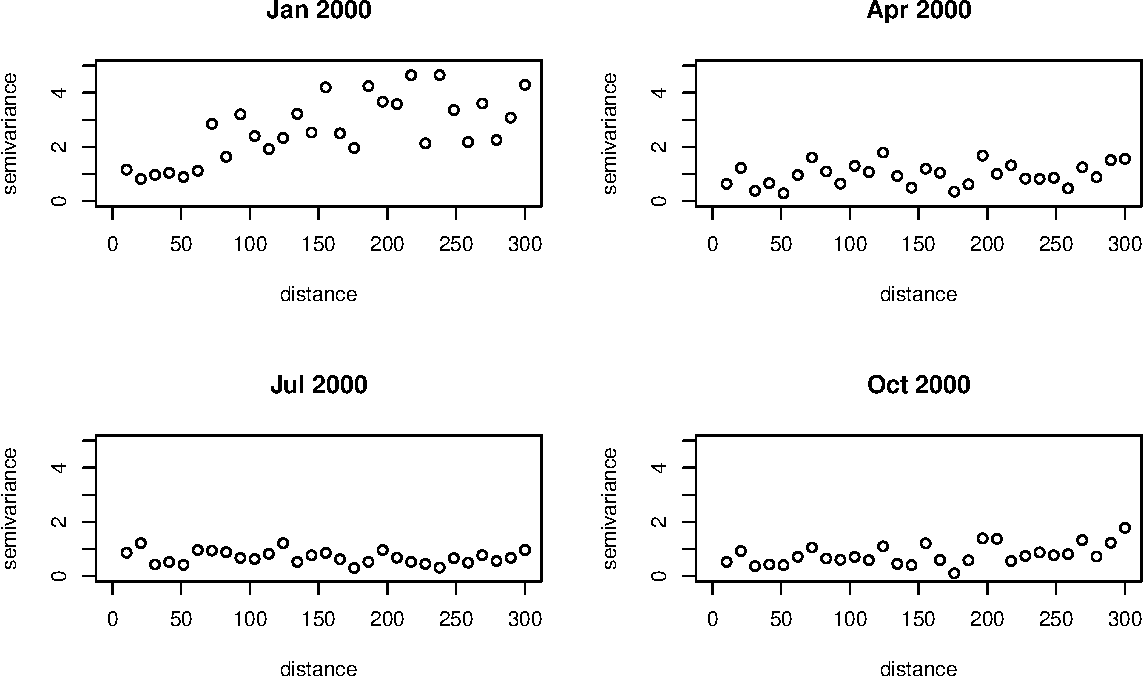
\includegraphics{Lec23_files/figure-beamer/unnamed-chunk-3-1.pdf}

\end{frame}

\begin{frame}[fragile]{Data and Model Parameters}

**Data*: \scriptoutput

\begin{Shaded}
\begin{Highlighting}[]
\NormalTok{coords =}\StringTok{ }\NormalTok{ne_temp }\OperatorTok\StringTok{ }\KeywordTok{select}\NormalTok{(UTMX, UTMY) }\OperatorTok\StringTok{ }\KeywordTok{as.matrix}\NormalTok{() }\OperatorTok{/}\StringTok{ }\DecValTok{1000}
\NormalTok{y_t =}\StringTok{ }\NormalTok{ne_temp }\OperatorTok\StringTok{ }\KeywordTok{select}\NormalTok{(}\KeywordTok{starts_with}\NormalTok{(}\StringTok{"y."}\NormalTok{)) }\OperatorTok\StringTok{ }\KeywordTok{as.matrix}\NormalTok{()}

\NormalTok{max_d =}\StringTok{ }\NormalTok{coords }\OperatorTok\StringTok{ }\KeywordTok{dist}\NormalTok{() }\OperatorTok\StringTok{ }\KeywordTok{max}\NormalTok{()}
\NormalTok{n_t =}\StringTok{ }\KeywordTok{ncol}\NormalTok{(y_t)}
\NormalTok{n_s =}\StringTok{ }\KeywordTok{nrow}\NormalTok{(y_t)}
\end{Highlighting}
\end{Shaded}

**Parameters*: \scriptoutput

\begin{Shaded}
\begin{Highlighting}[]
\NormalTok{n_beta =}\StringTok{ }\DecValTok{2}
\NormalTok{starting =}\StringTok{ }\KeywordTok{list}\NormalTok{(}
  \DataTypeTok{beta =} \KeywordTok{rep}\NormalTok{(}\DecValTok{0}\NormalTok{, n_t }\OperatorTok{*}\StringTok{ }\NormalTok{n_beta), }\DataTypeTok{phi =} \KeywordTok{rep}\NormalTok{(}\DecValTok{3}\OperatorTok{/}\NormalTok{(max_d}\OperatorTok{/}\DecValTok{2}\NormalTok{), n_t),}
  \DataTypeTok{sigma.sq =} \KeywordTok{rep}\NormalTok{(}\DecValTok{1}\NormalTok{, n_t), }\DataTypeTok{tau.sq =} \KeywordTok{rep}\NormalTok{(}\DecValTok{1}\NormalTok{, n_t), }
  \DataTypeTok{sigma.eta =} \KeywordTok{diag}\NormalTok{(}\FloatTok{0.01}\NormalTok{, n_beta)}
\NormalTok{)}

\NormalTok{tuning =}\StringTok{ }\KeywordTok{list}\NormalTok{(}\DataTypeTok{phi =} \KeywordTok{rep}\NormalTok{(}\DecValTok{1}\NormalTok{, n_t))}

\NormalTok{priors =}\StringTok{ }\KeywordTok{list}\NormalTok{(}
  \DataTypeTok{beta.0.Norm =} \KeywordTok{list}\NormalTok{(}\KeywordTok{rep}\NormalTok{(}\DecValTok{0}\NormalTok{, n_beta), }\KeywordTok{diag}\NormalTok{(}\DecValTok{1000}\NormalTok{, n_beta)), }
  \DataTypeTok{phi.Unif =} \KeywordTok{list}\NormalTok{(}\KeywordTok{rep}\NormalTok{(}\DecValTok{3}\OperatorTok{/}\NormalTok{(}\FloatTok{0.9} \OperatorTok{*}\StringTok{ }\NormalTok{max_d), n_t), }\KeywordTok{rep}\NormalTok{(}\DecValTok{3}\OperatorTok{/}\NormalTok{(}\FloatTok{0.05} \OperatorTok{*}\StringTok{ }\NormalTok{max_d), n_t)), }
  \DataTypeTok{sigma.sq.IG =} \KeywordTok{list}\NormalTok{(}\KeywordTok{rep}\NormalTok{(}\DecValTok{2}\NormalTok{, n_t), }\KeywordTok{rep}\NormalTok{(}\DecValTok{2}\NormalTok{, n_t)), }
  \DataTypeTok{tau.sq.IG =} \KeywordTok{list}\NormalTok{(}\KeywordTok{rep}\NormalTok{(}\DecValTok{2}\NormalTok{, n_t), }\KeywordTok{rep}\NormalTok{(}\DecValTok{2}\NormalTok{, n_t)),}
  \DataTypeTok{sigma.eta.IW =} \KeywordTok{list}\NormalTok{(}\DecValTok{2}\NormalTok{, }\KeywordTok{diag}\NormalTok{(}\FloatTok{0.001}\NormalTok{, n_beta))}
\NormalTok{)}
\end{Highlighting}
\end{Shaded}

\end{frame}

\begin{frame}[fragile]{Fitting with \texttt{spDynLM} from
\texttt{spBayes}}

\scriptoutput

\begin{Shaded}
\begin{Highlighting}[]
\NormalTok{n_samples =}\StringTok{ }\DecValTok{10000}
\NormalTok{models =}\StringTok{ }\KeywordTok{lapply}\NormalTok{(}\KeywordTok{paste0}\NormalTok{(}\StringTok{"y."}\NormalTok{,}\DecValTok{1}\OperatorTok{:}\DecValTok{24}\NormalTok{, }\StringTok{"~elev"}\NormalTok{), as.formula)}

\NormalTok{m =}\StringTok{ }\KeywordTok{spDynLM}\NormalTok{(}
\NormalTok{  models, }\DataTypeTok{data =}\NormalTok{ ne_temp, }\DataTypeTok{coords =}\NormalTok{ coords, }\DataTypeTok{get.fitted =} \OtherTok{TRUE}\NormalTok{,}
  \DataTypeTok{starting =}\NormalTok{ starting, }\DataTypeTok{tuning =}\NormalTok{ tuning, }\DataTypeTok{priors =}\NormalTok{ priors,}
  \DataTypeTok{cov.model =} \StringTok{"exponential"}\NormalTok{, }\DataTypeTok{n.samples =}\NormalTok{ n_samples, }\DataTypeTok{n.report =} \DecValTok{1000}\NormalTok{)}

\KeywordTok{save}\NormalTok{(m, ne_temp, models, coords, starting, tuning, priors, n_samples, }
     \DataTypeTok{file=}\StringTok{"dynlm.Rdata"}\NormalTok{)}

\NormalTok{##  ----------------------------------------}
\NormalTok{##      General model description}
\NormalTok{##  ----------------------------------------}
\NormalTok{##  Model fit with 34 observations in 24 time steps.}
\NormalTok{##  }
\NormalTok{##  Number of missing observations 0.}
\NormalTok{##  }
\NormalTok{##  Number of covariates 2 (including intercept if specified).}
\NormalTok{##  }
\NormalTok{##  Using the exponential spatial correlation model.}
\NormalTok{##  }
\NormalTok{##  Number of MCMC samples 10000.}
\NormalTok{##}
\NormalTok{##  ...}
\end{Highlighting}
\end{Shaded}

\end{frame}

\begin{frame}{Posterior Inference - \(\beta\)s}

\vspace{4mm}

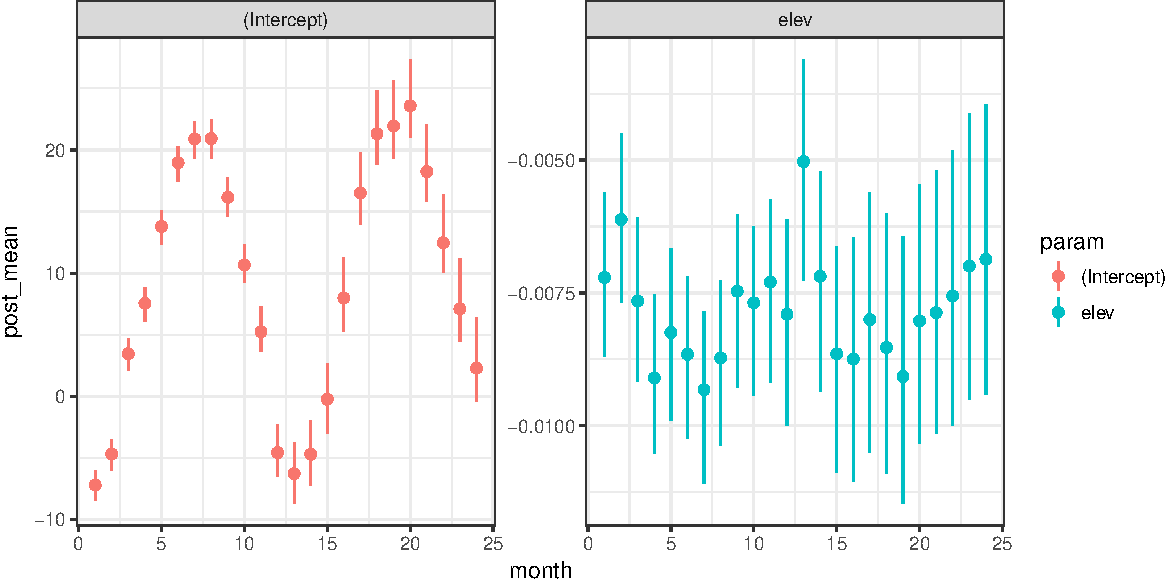
\includegraphics{Lec23_files/figure-beamer/unnamed-chunk-8-1.pdf}

\vvfill

\scriptsize

\href{https://en.wikipedia.org/wiki/Lapse_rate}{Lapse Rate}

\end{frame}

\begin{frame}{Posterior Inference - \(\theta\)}

\vspace{4mm}

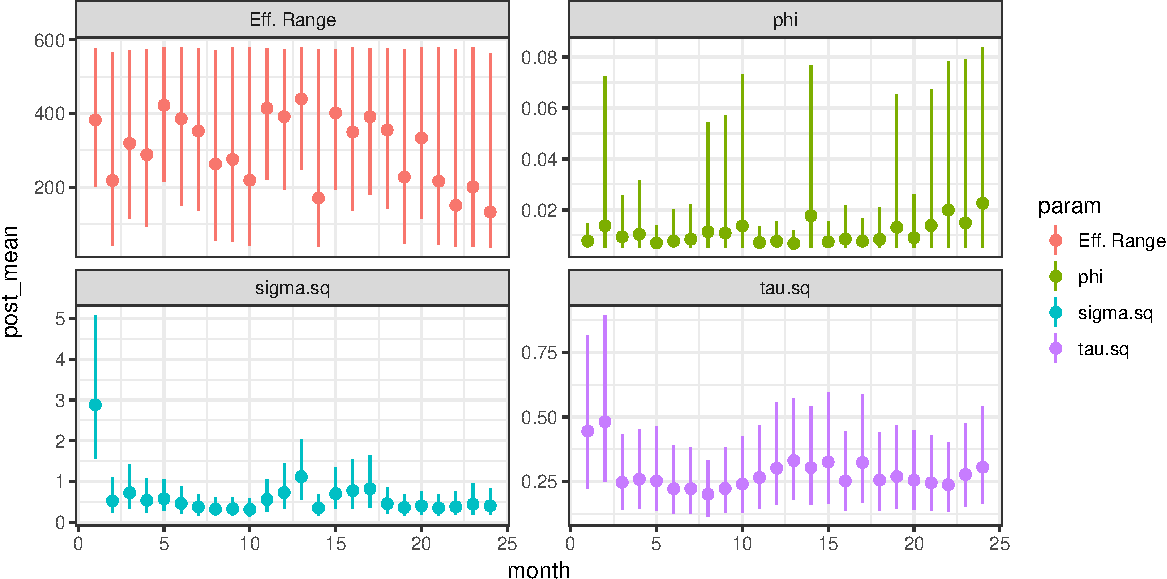
\includegraphics{Lec23_files/figure-beamer/unnamed-chunk-9-1.pdf}

\end{frame}

\begin{frame}{Posterior Inference - Observed vs.~Predicted}

\vspace{4mm}

\begin{center}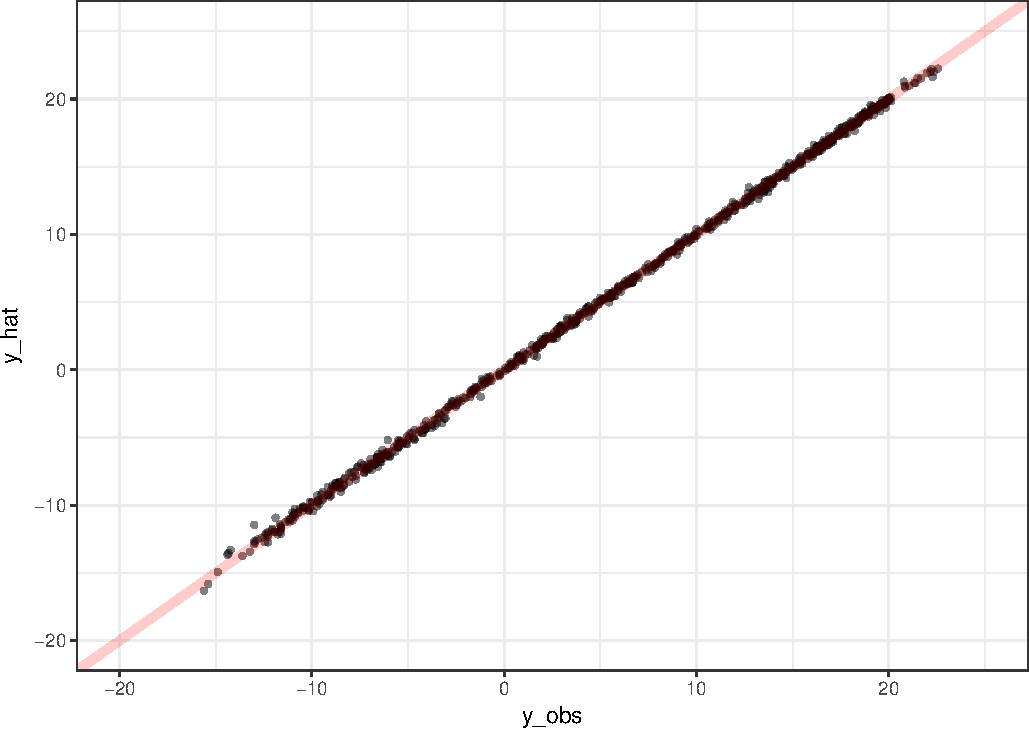
\includegraphics[width=\textwidth]{Lec23_files/figure-beamer/unnamed-chunk-10-1} \end{center}

\end{frame}

\begin{frame}[fragile]{Prediction}

\texttt{spPredict} does not support \texttt{spDynLM} objects.

\begin{Shaded}
\begin{Highlighting}[]
\NormalTok{r =}\StringTok{ }\KeywordTok{raster}\NormalTok{(}\DataTypeTok{xmn=}\FloatTok{575e4}\NormalTok{, }\DataTypeTok{xmx=}\FloatTok{630e4}\NormalTok{, }\DataTypeTok{ymn=}\FloatTok{300e4}\NormalTok{, }\DataTypeTok{ymx=}\FloatTok{355e4}\NormalTok{, }\DataTypeTok{nrow=}\DecValTok{20}\NormalTok{, }\DataTypeTok{ncol=}\DecValTok{20}\NormalTok{)}

\NormalTok{pred =}\StringTok{ }\KeywordTok{xyFromCell}\NormalTok{(r, }\DecValTok{1}\OperatorTok{:}\KeywordTok{length}\NormalTok{(r)) }\OperatorTok\StringTok{ }
\StringTok{  }\KeywordTok{cbind}\NormalTok{(}\DataTypeTok{elev=}\DecValTok{0}\NormalTok{, ., }\KeywordTok{matrix}\NormalTok{(}\OtherTok{NA}\NormalTok{, }\DataTypeTok{nrow=}\KeywordTok{length}\NormalTok{(r), }\DataTypeTok{ncol=}\DecValTok{24}\NormalTok{)) }\OperatorTok
\StringTok{  }\KeywordTok{as.data.frame}\NormalTok{() }\OperatorTok
\StringTok{  }\KeywordTok{setNames}\NormalTok{(}\KeywordTok{names}\NormalTok{(ne_temp)) }\OperatorTok
\StringTok{  }\KeywordTok{rbind}\NormalTok{(ne_temp, .) }\OperatorTok
\StringTok{  }\KeywordTok{select}\NormalTok{(}\DecValTok{1}\OperatorTok{:}\DecValTok{15}\NormalTok{) }\OperatorTok
\StringTok{  }\KeywordTok{select}\NormalTok{(}\OperatorTok{-}\NormalTok{elev)}
\end{Highlighting}
\end{Shaded}

\begin{Shaded}
\begin{Highlighting}[]
\NormalTok{models_pred =}\StringTok{ }\KeywordTok{lapply}\NormalTok{(}\KeywordTok{paste0}\NormalTok{(}\StringTok{"y."}\NormalTok{,}\DecValTok{1}\OperatorTok{:}\NormalTok{n_t, }\StringTok{"~1"}\NormalTok{), as.formula)}

\NormalTok{n_samples =}\StringTok{ }\DecValTok{5000}
\NormalTok{m_pred =}\StringTok{ }\KeywordTok{spDynLM}\NormalTok{(}
\NormalTok{  models_pred, }\DataTypeTok{data =}\NormalTok{ pred, }\DataTypeTok{coords =}\NormalTok{ coords_pred, }\DataTypeTok{get.fitted =} \OtherTok{TRUE}\NormalTok{,}
  \DataTypeTok{starting =}\NormalTok{ starting, }\DataTypeTok{tuning =}\NormalTok{ tuning, }\DataTypeTok{priors =}\NormalTok{ priors,}
  \DataTypeTok{cov.model =} \StringTok{"exponential"}\NormalTok{, }\DataTypeTok{n.samples =}\NormalTok{ n_samples, }\DataTypeTok{n.report =} \DecValTok{1000}\NormalTok{)}

\KeywordTok{save}\NormalTok{(m_pred, pred, models_pred, coords_pred, y_t_pred, n_samples, }
     \DataTypeTok{file=}\StringTok{"dynlm_pred.Rdata"}\NormalTok{)}
\end{Highlighting}
\end{Shaded}

\end{frame}

\begin{frame}{}

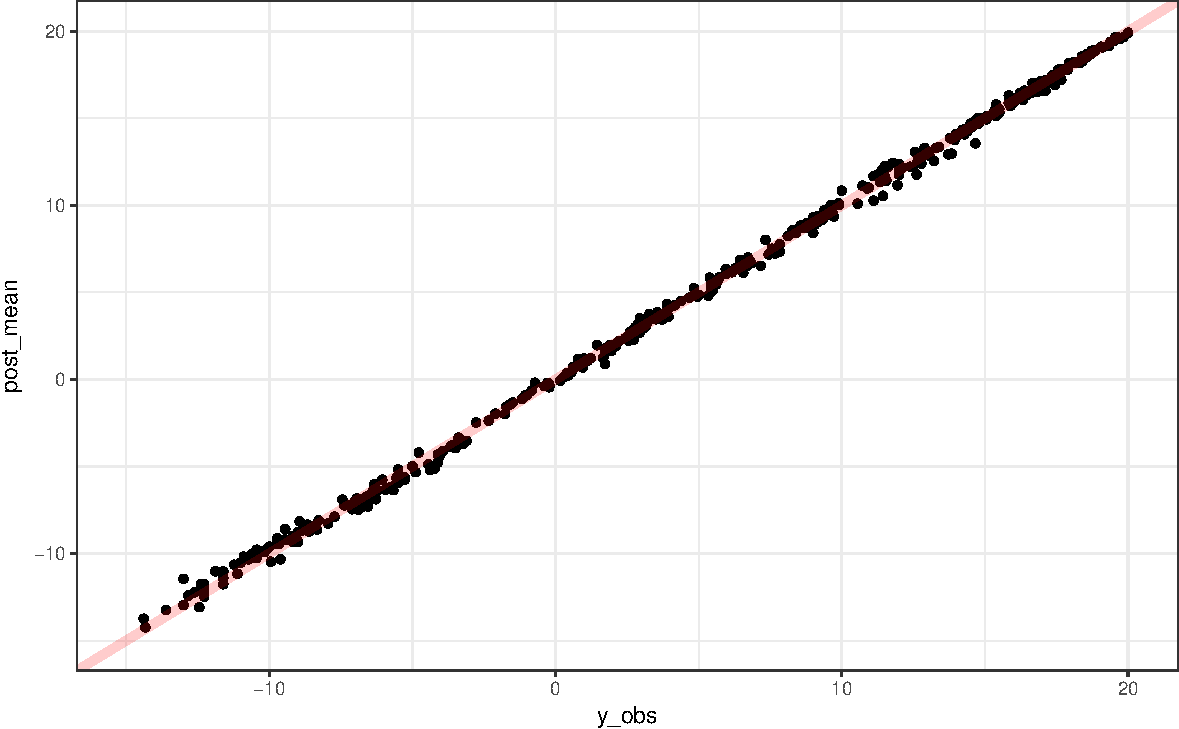
\includegraphics{Lec23_files/figure-beamer/unnamed-chunk-15-1.pdf}

\end{frame}

\begin{frame}{}

\begin{center}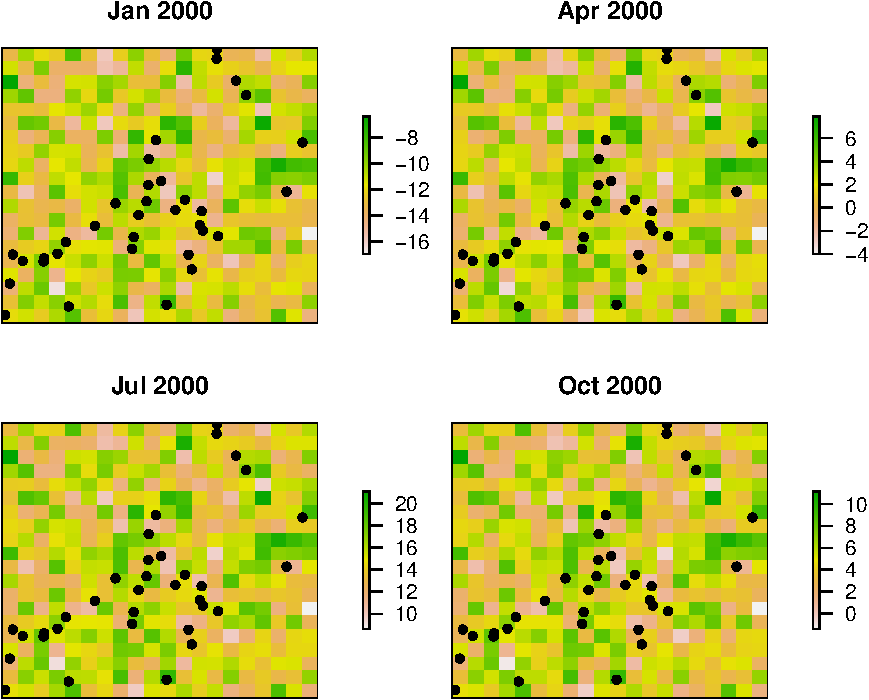
\includegraphics[width=0.8\textwidth]{Lec23_files/figure-beamer/unnamed-chunk-16-1} \end{center}

\end{frame}

\section{Spatio-temporal models for continuous
time}\label{spatio-temporal-models-for-continuous-time}

\begin{frame}[t]{Additive Models}

In general, spatiotemporal models will have a form like the following,

\[ \begin{aligned}
y(\bm{s},{t}) 
  &= \underset{\text{mean structure}}{\mu(\bm{s},{t})} + \underset{\text{error structure}}{{e}(\bm{s},{t})} \\
  &= \underset{\text{Regression}}{\bm{x}(\bm{s},{t}) \, \bm{\beta}(\bm{s},{t})} + \underset{\text{Spatiotemporal RE}}{{w}(\bm{s},{t})} + \underset{\text{Error}}{\epsilon(\bm{s},{t})}
\end{aligned} \]

\pause

\vspace{5mm}

The simplest possible spatiotemporal model is one were assume there is
no dependence between observations in space and time,

\[
w(\bm{s},t) = \alpha(t) + \omega(\bm{s})
\]

these are straight forward to fit and interpret but are quite limiting
(no shared information between space and time).

\end{frame}

\begin{frame}{Spatiotemporal Covariance}

Lets assume that we want to define our spatiotemporal random effect to
be a single stationary Gaussian Process (in 3 dimensions\(^\star\)),
\[ \bm{w}(\bm{s},\bm{t}) \sim \mathcal{N}\big(\bm{0}, \bm\Sigma(\bm{s},\bm{t})\big) \]
where our covariance function depends on both \(\lVert s-s'\rVert\) and
\(\lvert t-t'\rvert\), \[
\text{cov}(\bm{w}(\bm{s},\bm{t}), \bm{w}(\bm{s}',\bm{t}')) = c(\lVert s-s'\rVert, \lvert t-t'\rvert)
\]

\begin{itemize}
\item
  Note that the resulting covariance matrix \(\Sigma\) will be of size
  \(n_s \cdot n_t \times n_s \cdot n_t\).

  \begin{itemize}
  \item
    Even for modest problems this gets very large (past the point of
    direct computability).
  \item
    If \(n_t = 52\) and \(n_s = 100\) we have to work with a
    \(5200 \times 5200\) covariance matrix
  \end{itemize}
\end{itemize}

\end{frame}

\begin{frame}{Separable Models}

One solution is to use a seperable form, where the covariance is the
product of a valid 2d spatial and a valid 1d temporal covariance /
correlation function, \[
\text{cov}(\bm{w}(\bm{s},\bm{t}), \bm{w}(\bm{s}',\bm{t}')) = \sigma^2 \, \rho_1(\lVert \bm{s}-\bm{s}'\rVert;\bm\theta) \, \rho_2(\lvert \bm{t}-\bm{t}' \rvert; \bm{\phi})
\]

\pause

If we define our observations as follows (stacking time locations within
spatial locations) \scriptsize
\[
\bm{w}^t_{\bm{s}} = \big(
  w(s_1,t_1)     ,\, \cdots ,\, w(s_1,t_{n_t}) ,\,
  w(s_2,t_1)     ,\, \cdots ,\, w(s_2,t_{n_t}) ,\, \cdots ,\, \cdots ,\,
  w(s_{n_s},t_1) ,\, \cdots ,\, w(s_{n_s},t_{n_t}) \big)
\] \normalsize
then the covariance can be written as \[
\bm\Sigma_w(\sigma^2, \theta, \phi) = \sigma^2 \, \bm{H}_s(\theta) \otimes \bm{H}_t(\phi)
\] where \(\bm{H}_s(\theta)\) and \(\bm{H}_t(\theta)\) are
\(n_s \times n_s\) and \(n_t \times n_t\) sized correlation matrices
respectively and their elements are defined by \footnotesize
\[\begin{aligned}
\{\bm{H}_s(\theta)\}_{ij} &= \rho_1(\lVert \bm{s}_i - \bm{s}_j \rVert; \theta) \\
\{\bm{H}_t(\phi)\}_{ij} &= \rho_1(\lvert t_i - t_j \rvert; \phi) \\
\end{aligned}\]

\end{frame}

\begin{frame}{Kronecker Product}

Definition: \[\begin{aligned}
\underset{[m \times n]}{\bm{A}} \otimes \underset{[p \times q]}{\bm{B}} = \underset{[m \cdot p \times  n \cdot q]}{\begin{pmatrix}
a_{11} \bm{B} & \cdots & a_{1n} \bm{B} \\
\vdots        & \ddots & \vdots        \\
a_{m1} \bm{B} & \cdots & a_{mn} \bm{B} \\
\end{pmatrix}}
\end{aligned}\]

\vspace{4mm}

\pause

Properties: \[\begin{aligned}
\bm{A} \otimes \bm{B}       &\ne \bm{B} \otimes \bm{A}  \qquad\text{(usually)} \\
\vspace{3mm}
(\bm{A} \otimes \bm{B})^t   &= \bm{A}^t \otimes \bm{B}^t \\
\vspace{3mm}
\det(\bm{A} \otimes \bm{B}) &= \det(\bm{B} \otimes \bm{A}) \\
&=\det(\bm{A})^{\text{rank}(\bm{B})} \det(\bm{B})^{\text{rank}(\bm{A})} \\
\vspace{3mm}
(\bm{A} \otimes \bm{B})^{-1} &= \bm{A}^{-1} \bm{B}^{-1}
\end{aligned}\]

\end{frame}

\begin{frame}{Kronecker Product and MVN Likelihoods}

If we have a spatiotemporal random effect with a separable form, \[
\bm{w}(\bm{s},\bm{t}) \sim \mathcal{N}(\bm{0},\, \bm\Sigma_w)
\] \[
\bm\Sigma_w = \sigma^2 \, \bm{H}_s \otimes \bm{H}_t
\]

then the likelihood for \(\bm{w}\) is given by

\[
-\frac{n}{2}\log 2\pi - \frac{1}{2} \log |\Sigma_w| - \frac{1}{2} \bm{w}^t \bm{\Sigma_w}^{-1} \bm{w}
\] \[
= -\frac{n}{2}\log 2\pi - \frac{1}{2} \log \left[ (\sigma^2)^{n_t \cdot n_s} |H_s|^{n_t} |H_t|^{n_s}\right] - \frac{1}{2} \bm{w}^t \frac{1}{\sigma^2}(\bm{H}_s^{-1} \otimes \bm{H}_t^{-1}) \bm{w}
\]

\end{frame}

\begin{frame}[t]{Non-seperable Models}

\begin{itemize}
\tightlist
\item
  Additive and separable models are still somewhat limiting
\end{itemize}

\vspace{2mm}

\begin{itemize}
\tightlist
\item
  Cannot treat spatiotemporal covariances as 3d observations
\end{itemize}

\vspace{2mm}

\begin{itemize}
\item
  Possible alternatives:

  \begin{itemize}
  \tightlist
  \item
    Specialized spatiotemporal covariance functions, i.e. \[ 
    c(\bm{s}-\bm{s}', t-t') 
    = \sigma^2 (\lvert t - t'\rvert+1)^{-1} \exp\big(-\lVert\bm{s}-\bm{s}'\rVert (\lvert t-t' \rvert + 1)^{-\beta/2}\big)
    \] \[ ~ \]
  \item
    Mixtures, i.e. \(w(\bm{s},t) = w_1(\bm{s},t) + w_2(\bm{s},t)\),
    where \(w_1(\bm{s},t)\) and \(w_2(\bm{s},t)\) have seperable forms.
  \end{itemize}
\end{itemize}

\end{frame}

\end{document}
